%-------------------------------------------------------------------------------
\section{Accuracy Analysis}
\label{sec:accuracy}
%-------------------------------------------------------------------------------

\begin{figure*}[t]
    \centering
    \begin{subfigure}[b]{0.325\linewidth}
        \centering
        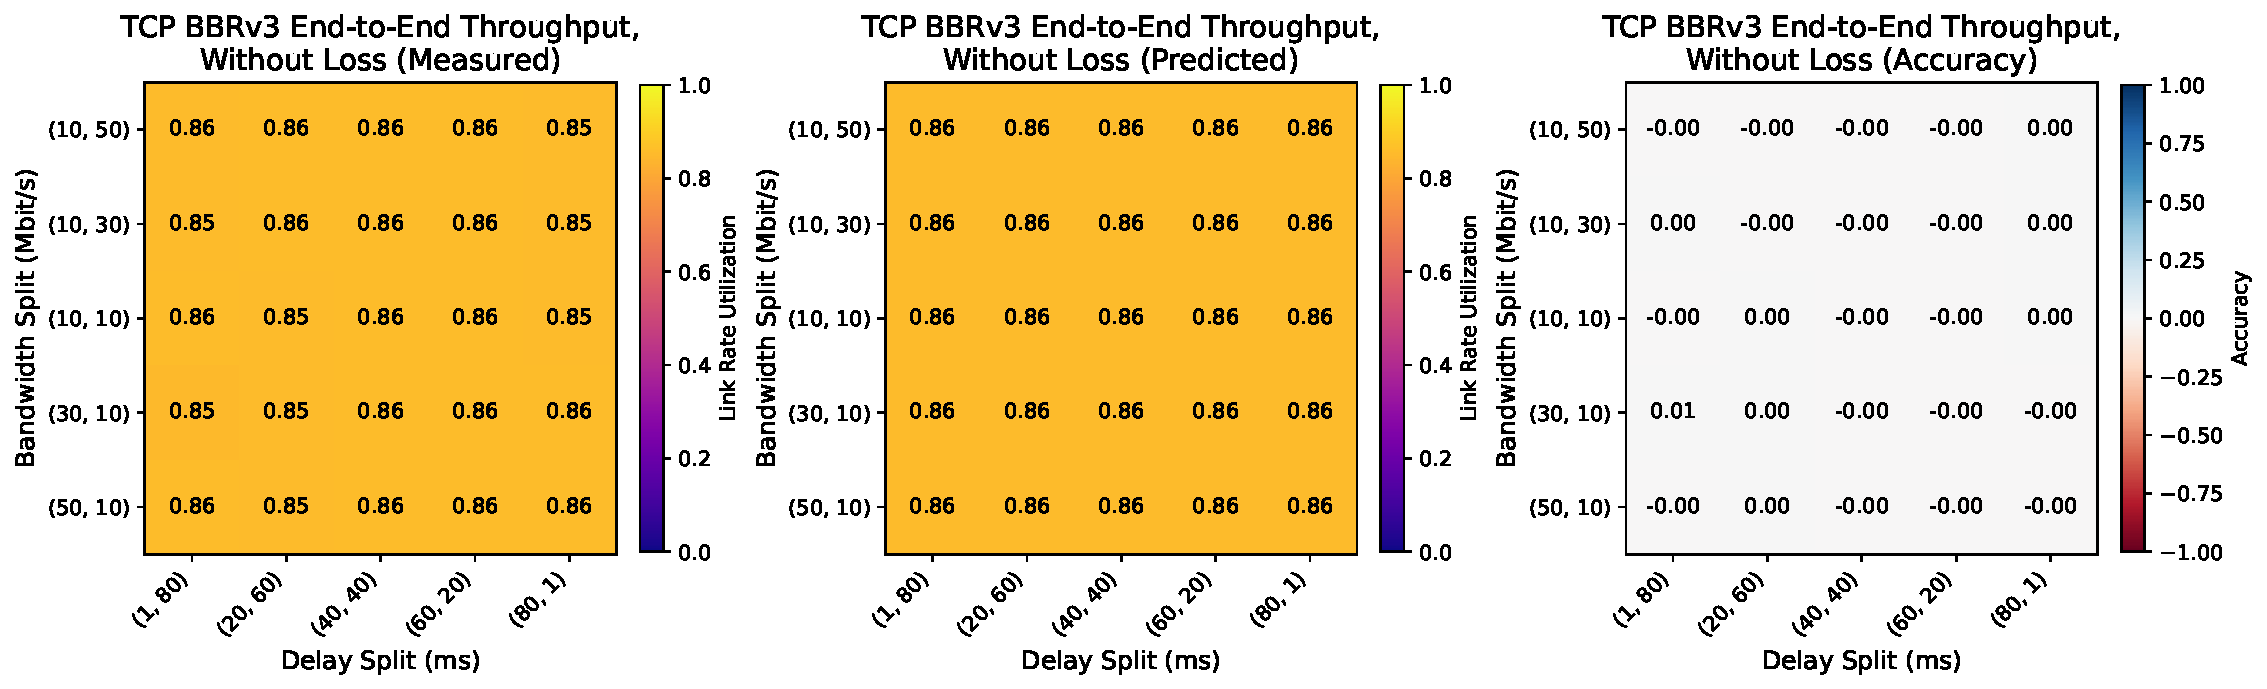
\includegraphics[width=\linewidth,trim={0 0 25.8cm 0},clip]
         {splitting-paper/figures/accuracy/accuracy_e2e_without_loss.pdf}
        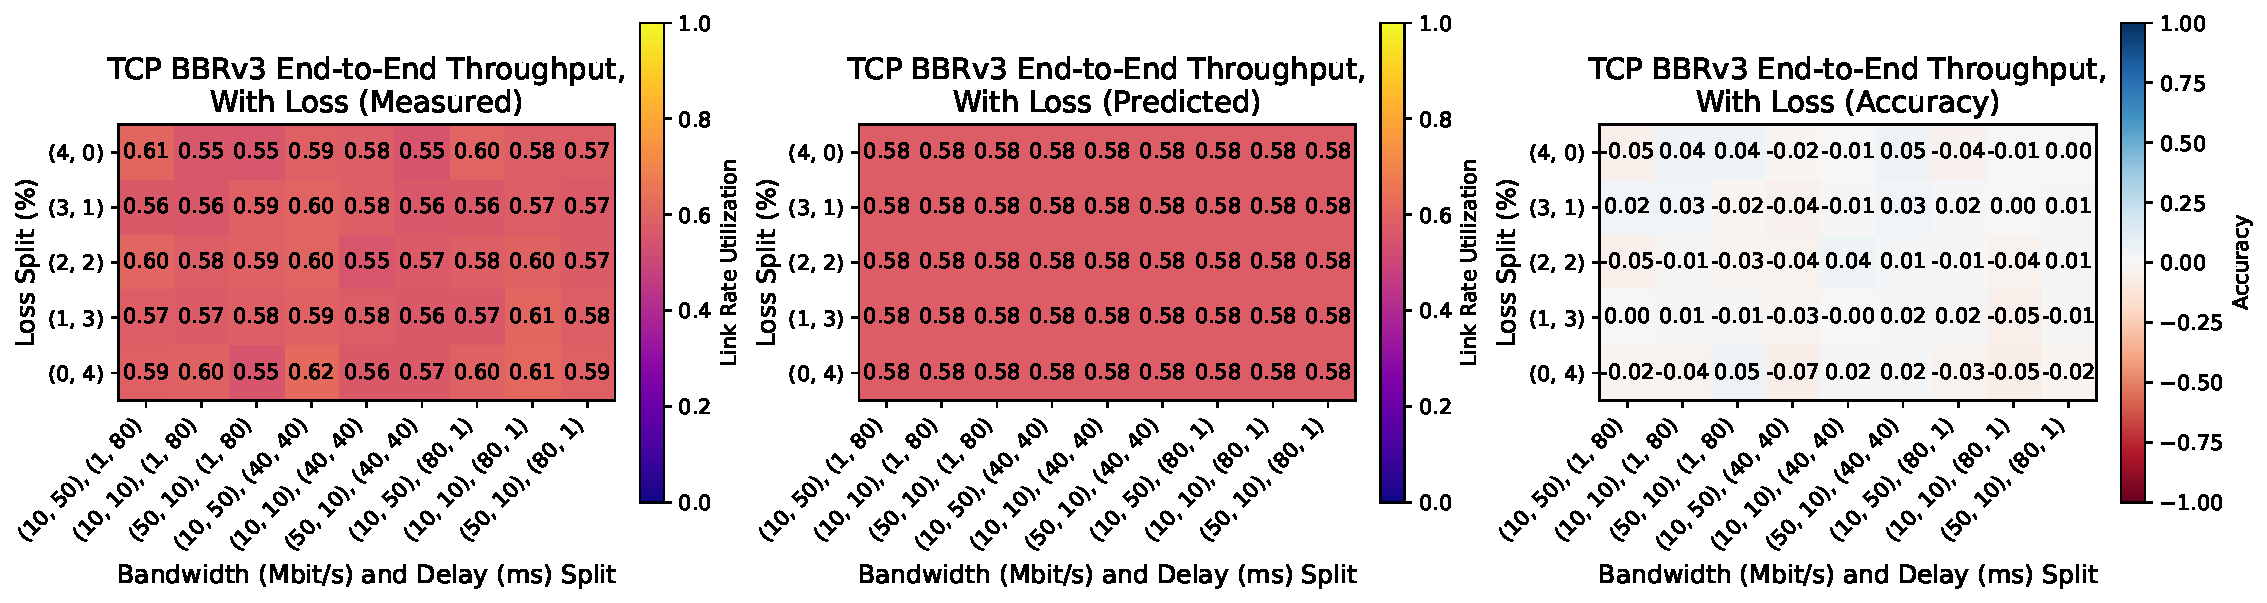
\includegraphics[width=\linewidth,trim={0 0 25.8cm 0},clip]
         {splitting-paper/figures/accuracy/accuracy_e2e_with_loss.pdf}
        \captionsetup{skip=4pt}
        \caption{End-to-end throughput accuracy.}
        \label{fig:accuracy:e2e}
    \end{subfigure}
    \begin{subfigure}[b]{0.645\linewidth}
        \centering
        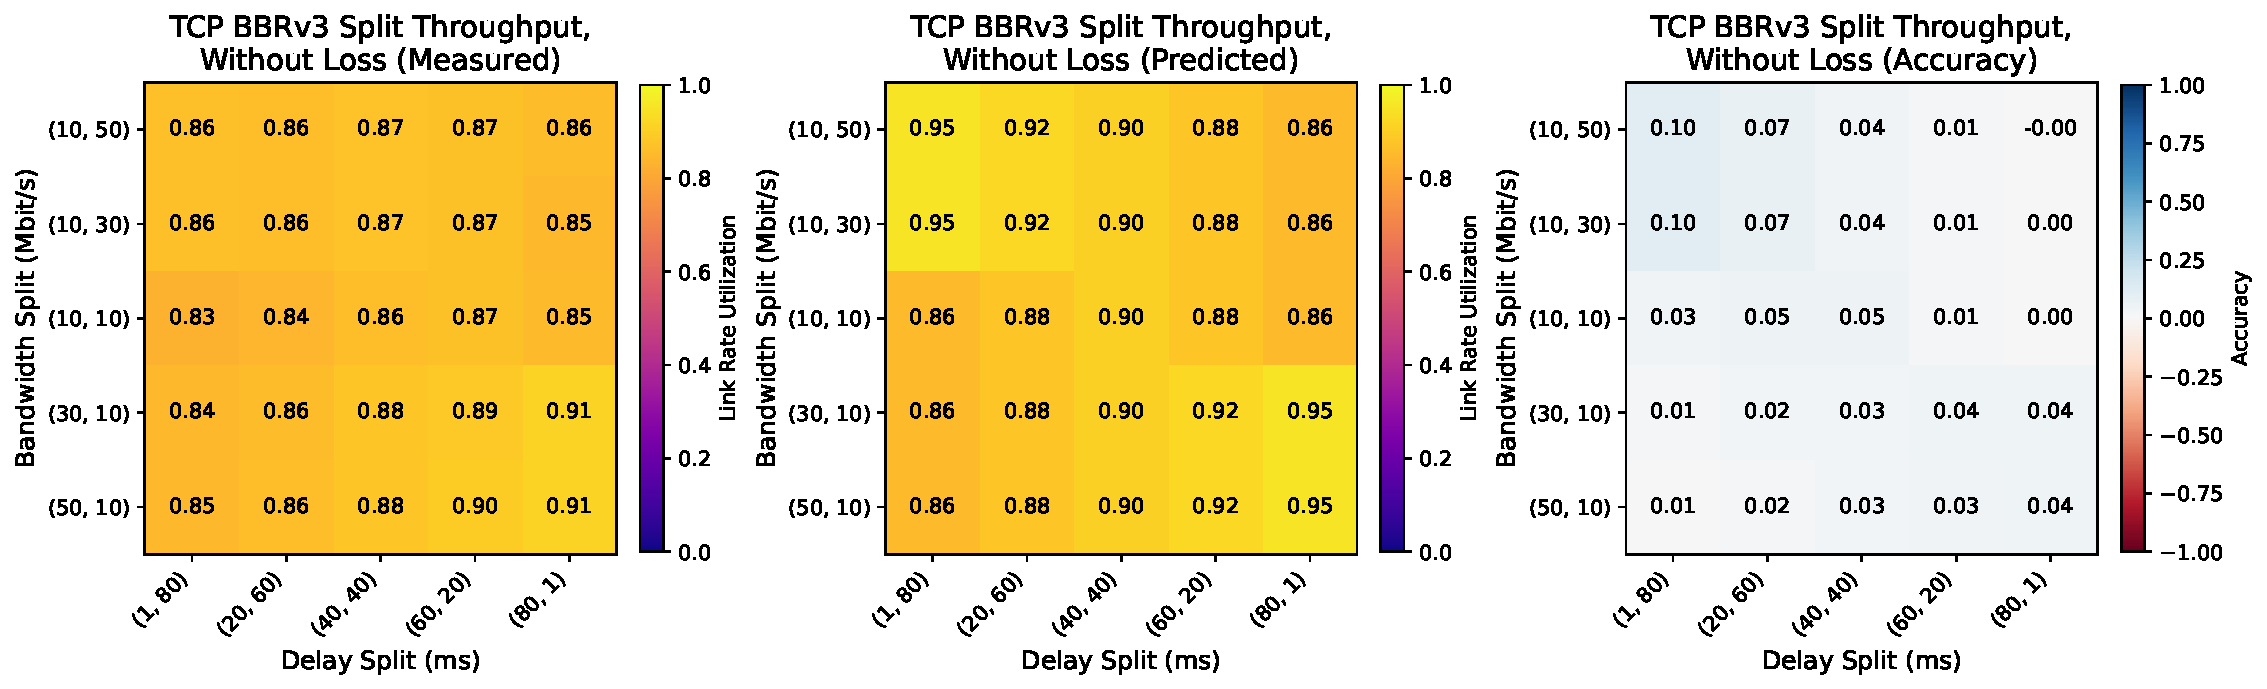
\includegraphics[width=\linewidth,trim={0 0 13.4cm 0},clip]
         {splitting-paper/figures/accuracy/accuracy_split_without_loss.pdf}
        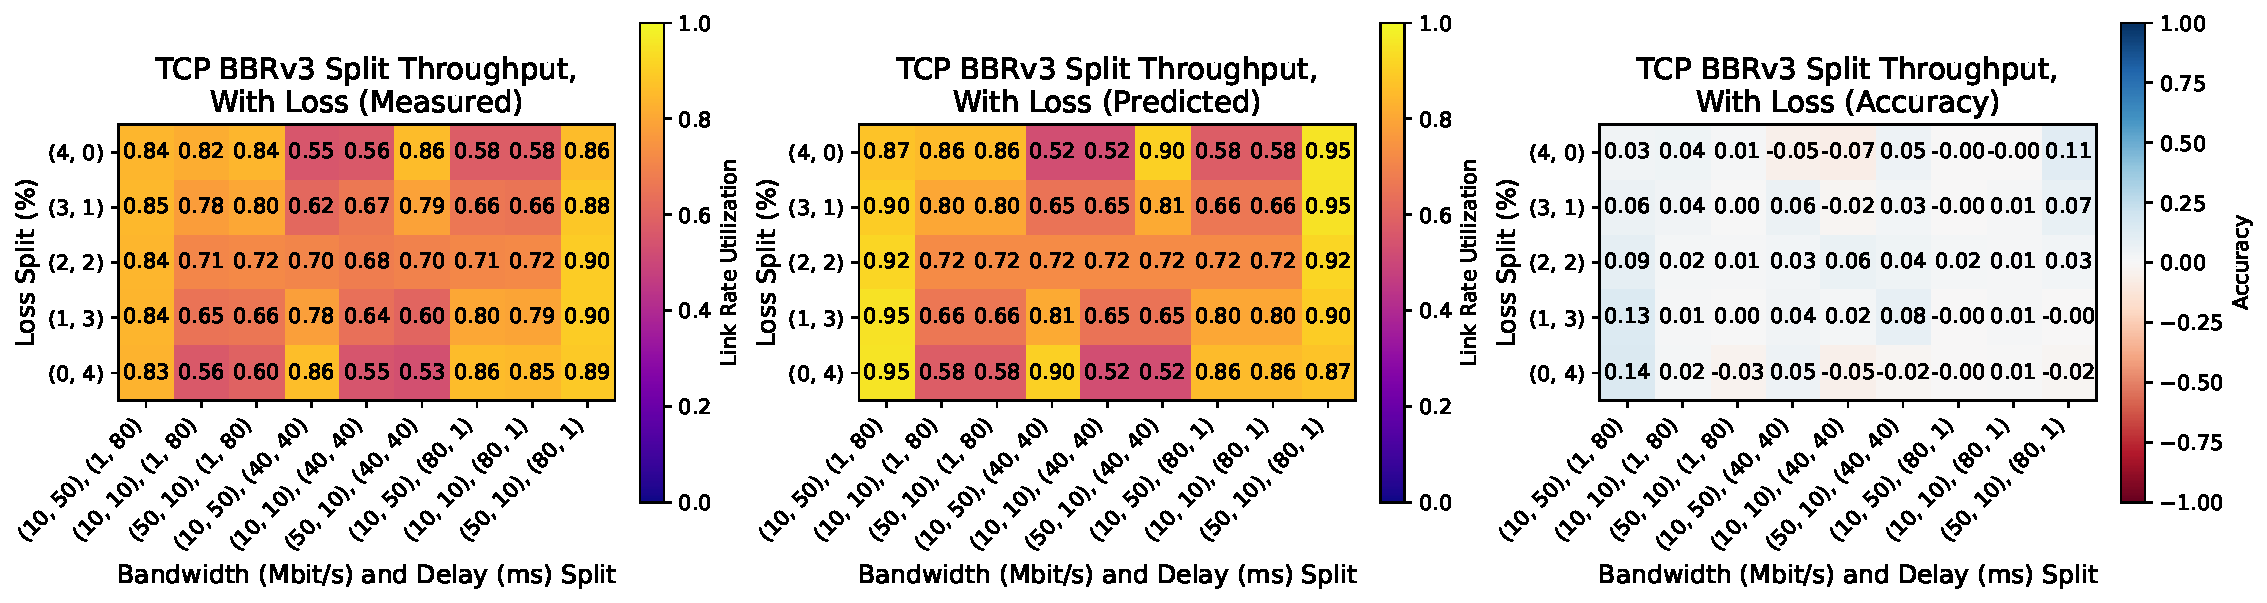
\includegraphics[width=\linewidth,trim={0 0 13.4cm 0},clip]
         {splitting-paper/figures/accuracy/accuracy_split_with_loss.pdf}
        \captionsetup{skip=4pt}
        \caption{Split throughput accuracy.}
        \label{fig:accuracy:split}
    \end{subfigure}

    \caption{Heatmaps of the measured and predicted BBRv3 throughputs for
     various splits of delay, bandwidth, and loss, both without (top) and with
     (bottom) loss.
     The \textit{end-to-end throughput} predictions (not pictured) are the same for all
     cells at 0.86 utilization without loss and 0.58 utilization with loss,
     because they represent the same network path, so end-to-end
     prediction errors are roughly uniform.
     The \textit{split throughput} predictions err slightly on the side of
     overestimation, but they accurately reflect trends in higher or lower throughputs for
     measurements on different splits of the same network path. Median of $n=40$ trials.}
    \label{fig:accuracy}
    \vspace{-0.3cm}
\end{figure*}


Our analysis of connection-splitting for TCP and its extensions to QUIC rely on
the accuracy of the split throughput heuristic. In this section, we are
primarily concerned with how accurate our predictions, which are based on
measurements from a one-segment topology, are for measurements from a
two-segment topology in emulation, without and with a connection-splitting TCP
PEP:
\begin{itemize}[noitemsep]
\item Does the \texttt{compose} function accurately represent the combined
 network path in the end-to-end throughput?
\item Does the split throughput heuristic accurately predict split throughput?
\end{itemize}

\noindent Most importantly, we find the heuristic to be able to usefully
 predict \textit{trends}.
 In terms of absolute predictions, we find the \texttt{pred\_e2e\_throughput()}
 and \texttt{pred\_split\_throughput()} functions to be correct within a
 reasonable tolerance, with a slight tendency to overestimate.
 % the \texttt{pred\_e2e\_throughput()} function enables
 % us to predict emulated end-to-end throughput within $7$\% and the \texttt
 % {pred\_split\_throughput()} function within $14$\%.

Orthogonally, we do not evaluate the accuracy to which emulation studies reflect
the real world with multi-flow settings and more complex network properties,
nor how the accuracy would extrapolate to QUIC connections with custom
connection splitters. It may be interesting to explore how to incorporate
such factors into the network model and heuristic.

\paragraph{Methodology.} Recall that for a given network path composed of two
 path segments, we can obtain both the predicted end-to-end and split
 throughputs, and the ground truth throughputs in an emulated network with and
 without a TCP PEP. Then for a network setting, we can compute the accuracy as
 the percent error in predicted vs. measured throughput.

We perform an empirical accuracy analysis of BBRv3 for two end-to-end network paths with
identical bandwidth and delay, both without (0\%) and with (4\%) loss. We test
various splits for the bandwidth, delay, and loss and analyze the accuracy
trends. In particular, we select delay splits such that the end-to-end delay is
80 ms, bandwidth splits such that the bottleneck bandwidth is 10 Mbit/s, and loss
splits such that the total loss is either 0\% or 4\%. We parameterize the network
path segments to use the cached measurements from \Cref
{tab:parameters}.

\subsection{End-to-End Throughput Accuracy}

Each of our splits composes to the same end-to-end network path, so we predict
the same end-to-end throughput for each. Our experimental
results in \Cref{fig:accuracy:e2e} show that the measured end-to-end
throughputs are also roughly uniform, especially without loss, indicating that
our method of composing network path segments in emulation represents the same
end-to-end network path.

\subsection{Split Throughput Accuracy}

The split throughput predictions accurately reflect trends in loss, delay, and
bandwidth (\Cref{fig:accuracy:split}). For example, split throughput is
generally higher when the high-bandwidth link is paired with high delay
(the yellow-est cells). It is also lower when the lossy link is paired with
high delay (columns 1 and 2) or low bandwidth (columns 3-5).

The split throughput predictions tend to slightly overestimate, but we think
the level of error is small enough to be helpful for informing real PEP
deployment. The maximum error is $\pm14\%$, and on average $\pm4\%$. This
dwarfs the measured gains in some situations, and rules out a large gain in
others.

One factor that may lead to overestimation of split throughput is the queue
behavior and the burstiness of the sender. With small queues and bursty
sending, we would expect the far path segment from the data sender to sometimes
be limited by the send buffer. This could subsequently affect how the far
connection probes for and utilizes available link rate capacity.

Another factor is the proximity of the bottleneck link to the sender. While
our heuristic does not account for this, the real split throughputs for
symmetric pairs of network paths (e.g., the left three and right three columns
in \Cref{fig:accuracy:split}), show that we slightly overestimate
when the low-bandwidth bottleneck link is far from the sender.
Based on our reasoning about queues, this would suggest that the far path
segment, already the bottleneck, is even further under-saturated.

Overall, we find our end-to-end and split throughput predictions to usefully
reflect relative trends and absolute throughput within a
reasonable tolerance. They are not intended to make claims about exact achievable
throughputs nor about the immediate utility of PEPs in the real world,
but simply to reason about how connection-splitting may impact
long-lived throughput in a simplified network model.

% \subsection{Possible Sources of Error}

% \gina{TODO: Simple experiment exploring the effects of queue discipline?}

% \paragraph{Modeling the network queue.} The bottleneck throughputs of each path
%  segment are taken assuming that the data sender of each TCP connection has
%  enough data to continuously saturate the connection when data needs to be
%  sent. Thus the throughput at the far path segment might be lower than
%  predicted when the queue isn't saturated. This could be if the queue is small
%  and drops packets when there are bursts.

% Reasons for overestimation would be, the effective RTT increases if there is
% buildup in the queue. Some algorithms aim to have some packets in the queue at
% any time. Bandwidth differences affect burstiness without pacing.

% \begin{figure}
%     \centering
%     \includegraphics[width=\linewidth,height=100pt]{figures/figure11a.png}
%     \includegraphics[width=\linewidth,height=100pt]{figures/figure11b.png}
%     \caption{Effect of different queue disciplines on BBRv3's end-to-end and
%      split throughput in a specific network setting. Or pick whichever one
%      showed differences. Sometimes short queues have an effect. \gina{I want to
%      run this experiment again I think it could be totally different with the
%      new topology, these results did not totally make sense anyway.}}
%     \label{fig:qdiscs}
% \end{figure}

% \paragraph{Queueing discipline.} We analyze the effect of different queueing
%  configurations on the heuristic as a possible explanation for these errors
%  (\Cref{fig:qdiscs}). Consider several different queue disciplines: RED, PIE,
%  droptail with a large buffer of 1 BDP, droptail with a small buffer of
%  $0.1\cdot$BDP. We also consider traffic policers that don't have a queue at
%  all.

% \subsection{Limitations}

% We can also add different representations of loss and how to compose them.

% We recognize that real split TCP deployments may use even more path segments,
% and the network model does not capture many of the nuances of real networks,
% and that queues may be configured with other behavior such as drop-tail at
% proxies.

% TCP is also not limited to bulk data transfers, and is used in a variety of
% settings where it is valuable to have reliable, ordered delivery. TCP PEPs can
% be useful in other ways like faster retransmission for low jitter. We hope the
% understanding of how these network conditions and this setup on congestion
% control behavior can help the reader extrapolate the effects of split TCP PEPs
% in their own deployments.
